\section{Experiment I: regime confidence and causal estimation}
\subsection{Data-generating process}
We generate a two-state Markov chain $z_t\in\{0,1\}$ with transition matrix
\[
A=\begin{pmatrix}0.97&0.03\\0.03&0.97\end{pmatrix}.
\]
For independent standard normal disturbances, the structural equations are
\begin{align}
C_t&=U^C_t,&X_t&=C_t+U^X_t,\\
Y_t&=\theta_{z_t}X_t+2C_t+U^Y_t,&
M_t&=\mu_{z_t}+1.3U^M_t.
\label{eq:diagnostic}
\end{align}
Here $C_t$ is a confounder, $X_t$ a treatment-like variable, $Y_t$ the outcome, and $M_t$ a regime emission. The coefficient $\theta_{z_t}$ is the known target. Nominal emission means are $\boldsymbol\mu=(-0.7,0.7)$ (mu), and $\boldsymbol\theta=(1,-1)$ except in the inactive setting, where $\boldsymbol\theta=(1,0)$.

Each of 200 replications uses 2,000 training and 1,000 test observations. Seeds are $20260906+r$ for index $r=0,\ldots,199$. Training regimes and nominal filter parameters are oracle inputs. This removes regime-fitting uncertainty to isolate filtering from identification. The test filter sees emissions only, not future outcomes or true test states.

\subsection{Estimators and interventions}
We compare pooled unadjusted regression, pooled regression with available confounder adjustment, regime-specific slopes selected by maximum filtered posterior, posterior-weighted slopes, and an oracle test-state selector. Available adjustment becomes unadjusted in the hidden-confounder scenario.

The settings are observed confounding, omitted confounding, reversal of emission means at the test boundary, and an inactive second mechanism. After emission reversal the filter still uses nominal parameters. This is deliberate misspecification, not retraining on the shifted distribution.

Primary loss is mean squared error (MSE) of the structural coefficient. Mean absolute error (MAE) is also reported because one loss can improve while another worsens. These are estimation losses, not trading accuracy, return, or Sharpe ratio.

\subsection{Results}
\begin{table}[htbp]\centering\small
\begin{tabular}{lrrrr}\toprule
Setting & Pooled & Hard & Soft & Oracle\\\midrule
Observed confounder & 1.0250 & 0.5033 & 0.3734 & 0.0010\\
Hidden confounder & 2.0478 & 1.4971 & 1.3651 & 1.0039\\
Emission shift & 1.0250 & 3.5009 & 2.8903 & 0.0010\\
Inactive second regime & 0.2568 & 0.1264 & 0.0939 & 0.0010\\
\bottomrule\end{tabular}
\caption{Mean coefficient MSE over 200 replications. Full losses and Monte Carlo errors appear in the appendix.}
\end{table}
With observed confounding, posterior averaging has MSE 0.3734 versus 0.5033 for hard selection. Its MAE is 0.3745 versus 0.2726 for hard selection. The MSE improvement does not support an unqualified claim of greater accuracy.

With hidden confounding, even the oracle selector has MSE approximately 1.004. Perfect regime knowledge does not remove omitted-variable bias. After emission reversal, the soft gate has MSE 2.8903, worse than the pooled adjusted value 1.0250. A filter can be confident under an incorrect mapping.

The inactive setting distinguishes an absent effect from an absent regime. A zero structural coefficient does not justify erasing that state's probability mass.
\begin{figure}[htbp]\centering
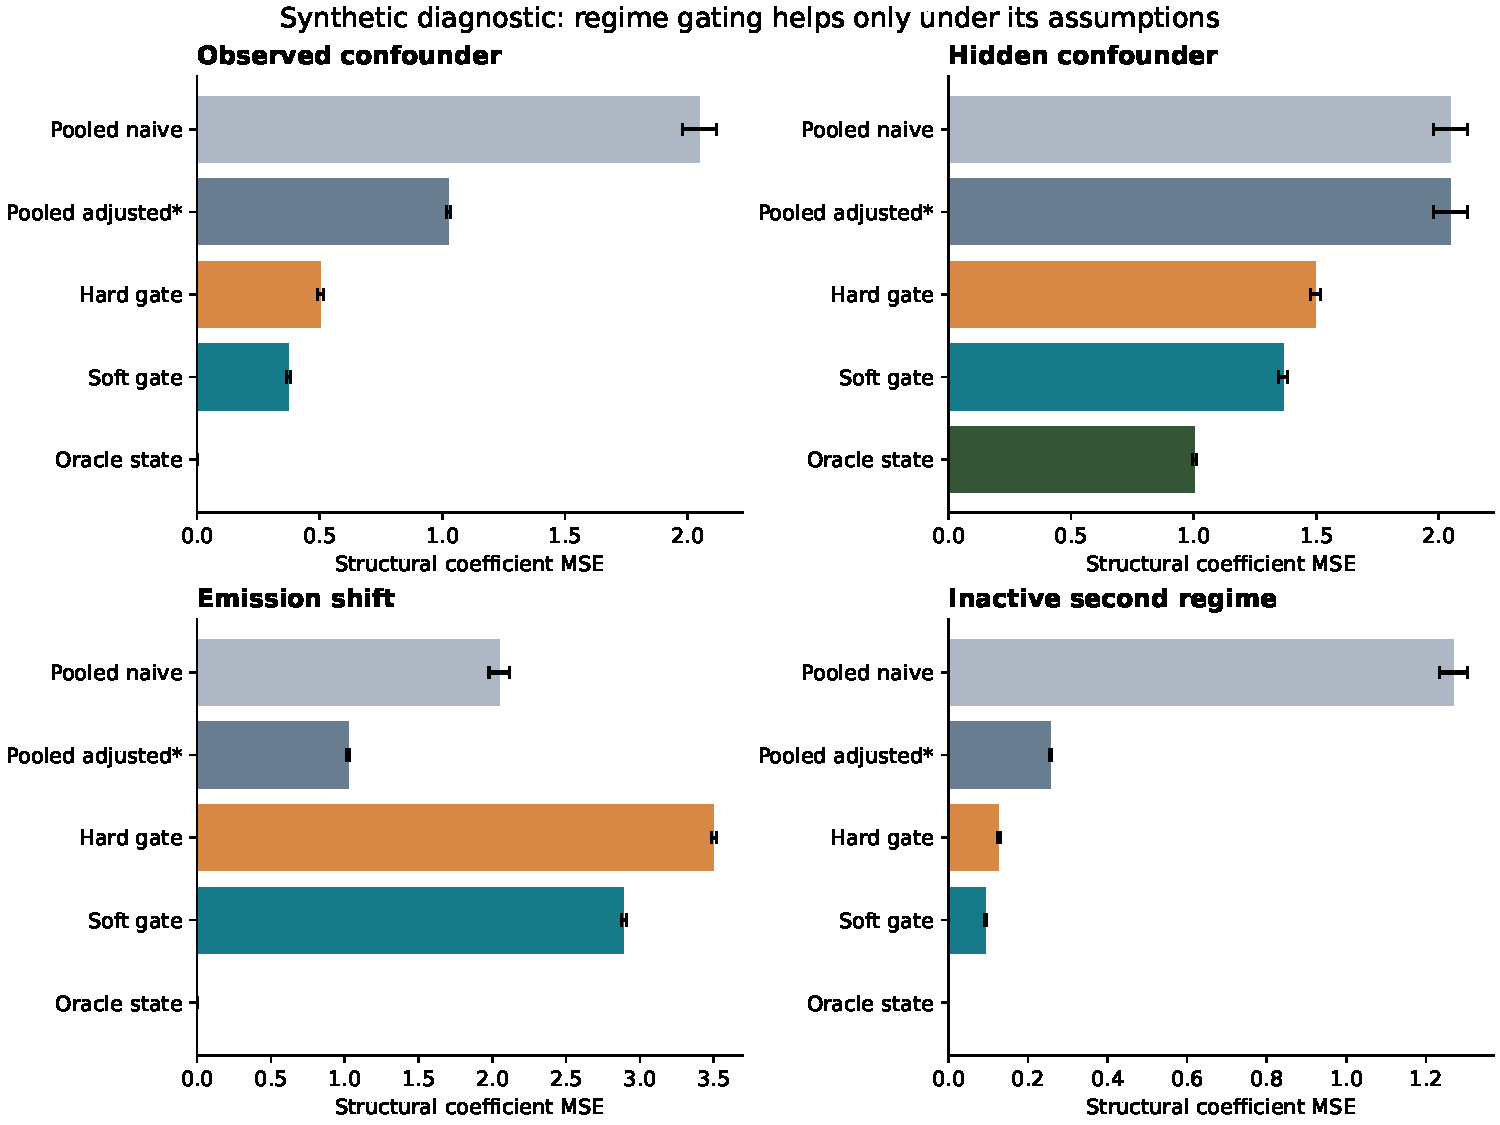
\includegraphics[width=.92\linewidth]{manuscript/figures/synthetic_results.pdf}
\caption{Structural-coefficient MSE. Error bars show 1.96 Monte Carlo standard errors across 200 replications, conditional on oracle training states and nominal filtering parameters. They do not quantify uncertainty about real financial mechanisms.}
\end{figure}

\section{Experiment II: interactive market feedback}
\subsection{Environment and neural proposals}
The environment contains 24 modeled participants over 360 steps. The first 60 steps initialize positions and state; the remaining 300 determine scored returns and stress events. A step has no calibrated duration in seconds, minutes, or trading days.

Two neural experts use 12 fixed tanh hidden features and ridge-fitted output layers. They learn $x$ and $-x$ from 4,096 separate training examples with noisy targets. Parameters are fixed during market tests. This is a compact random-feature neural model, not a large language model.

Participants receive a macro surprise $x_t$ with correlated measurement errors. A two-state posterior mixes the forecasts. Each policy includes the same momentum component. The simulator uses known nominal transition and emission parameters. True state influences the environment and evaluation but is not supplied as the policy's current label.

Let $p_t$ be log price, $F_t$ log fundamental proxy, $D_t$ normalized depth, and $\Delta h_{it}$ participant $i$'s position change. Returns follow
\begin{equation}
\Delta p_t=\operatorname{clip}\!\left(
\Delta F_t-\kappa(1-0.7\phi)(p_{t-1}-F_{t-1})
+\frac{\lambda\phi}{D_{t-1}}\overline{\Delta h}_t,\,-c_r,c_r\right).
\label{eq:market}
\end{equation}
Here $\kappa=0.06$ (kappa), $\lambda=0.012$, $c_r=0.25$, and the overbar averages modeled participants. A shock of zero or $-0.08$ enters the fundamental step at step 180. The numerical cap's binding frequency and sensitivity are reported.

Increasing $\phi$ changes two channels: order impact and background restoring pressure. Its measured effect is their joint effect. Separating them is a future factorial extension.

\subsection{Accounting, costs, and liquidity}
Targets are proportional to current marked wealth, leverage, and bounded signal. Adjustment is
\[
h_{it}=h_{i,t-1}+\eta(h^\star_{it}-h_{i,t-1}).
\]
Execution uses the arithmetic midpoint of pre- and post-update prices. Fees are 2 basis points of traded notional plus a spread term of $5/D_{t-1}$ basis points. These are stipulated values, not venue estimates.

Cash is debited for the order and cost; wealth equals cash plus marked position. Terminal liquidation charges the same cost convention, but its flow does not affect the terminal price. This simplification must be replaced before execution-capacity claims.

Depth evolves as
\[
D_t=\operatorname{clip}\!\left[
D_{t-1}+0.08(1-D_{t-1})-3|\Delta p_t|
-0.012\phi\,\overline{|\Delta h|}_t,\;0.12,\;1\right].
\]
It is an endogenous stress proxy, not observed book depth. No equation conserves background dealer inventory. Equal initial wealth and fixed participant count mean capital concentration is not varied in the completed experiment.

\subsection{Four policies and the factorial grid}
The ungated policy has neither liquidity cap nor evidence checks. The risk-only policy adds cap $\min(1,D/0.5)$ alone. The evidence-gated policy also checks timeliness, maximum regime probability at least 0.65, and lagged squared forecast error below 2.5. Wrong evidence reverses regime interpretation with the same checks and cap.

These checks are synthetic proxies. Timeliness uses a 5\% stale-information probability; a stale record is not a realistically delayed observation in this model. Forecast error is an exponentially weighted mean with update weight 0.05. A noisy outcome proxy arrives after orders for the next update.

The grid uses $\phi\in\{0,0.25,0.5,0.75\}$, $\rho\in\{0,0.85\}$, $\eta\in\{0.1,0.8\}$, $\ell\in\{1,3\}$, two shocks, and four policies: 256 configurations and 16,384 trajectories at 64 replications each. Common innovations support paired comparisons; all trajectories are not mutually independent.

\subsection{Results and attribution}
\begin{table}[htbp]\centering\small
\begin{tabular}{lrrrr}\toprule
Policy & Net return (\%) & Dislocation (\%) & No recovery (\%) & MSE\\\midrule
Ungated & -8.00 & 1.93 & 0.85 & 0.425\\
Risk only & -7.28 & 0.00 & 11.35 & 0.425\\
Evidence gate & -6.81 & 0.00 & 10.03 & 0.425\\
Wrong evidence & -2.80 & 0.00 & 0.00 & 2.962\\
\bottomrule\end{tabular}
\caption{Descriptive averages across the 64 base parameter settings per policy. These settings receive equal weight; this is not an estimated real-market distribution.}
\end{table}
Every policy has negative mean net return across the equally weighted grid. Evidence gating reduces mean losses versus the uncapped comparator, but risk-only also improves outcomes. Wrong evidence has the smallest average loss despite much worse forecast error. Its lower eligibility rate reduces exposure and trading.

Persistent absolute dislocations occur in some ungated configurations and none of the tested capped configurations. This cannot be attributed specifically to causal evidence: risk-only also removes these events in the tested grid. Zero observed events in 64 replications does not imply zero population risk.

The high-coupling, correlated, fast, leveraged shock scenario illustrates a conflict. Evidence gating has smaller losses and fewer price-drawdown events than the uncapped policy, but all its replications fail the specified joint recovery condition by horizon end. Individual loss control and collective recovery are different metrics.
\begin{figure}[htbp]\centering
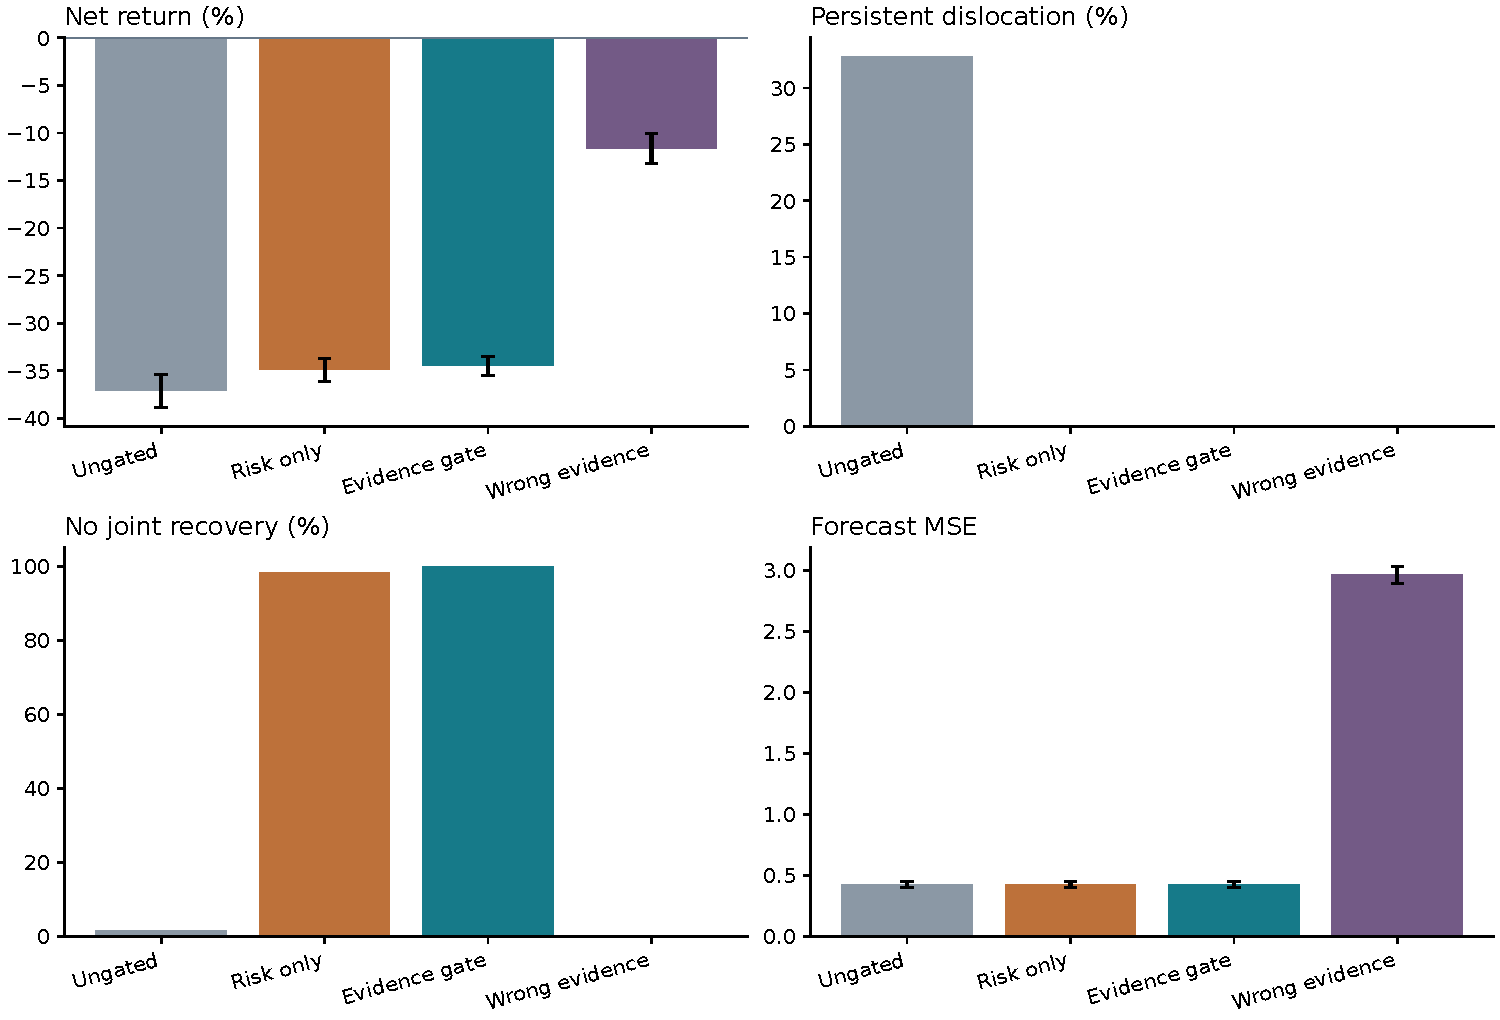
\includegraphics[width=\linewidth]{manuscript/figures/market_comparison.pdf}
\caption{Matched high-coupling shock scenario: $\phi=0.75$, $\rho=0.85$, $\eta=0.8$, $\ell=3$. Mean net return, persistent dislocation rate, joint recovery failure, and forecast MSE use the same 64 innovations per policy. Smaller losses do not establish better forecasts.}
\end{figure}
\begin{figure}[htbp]\centering
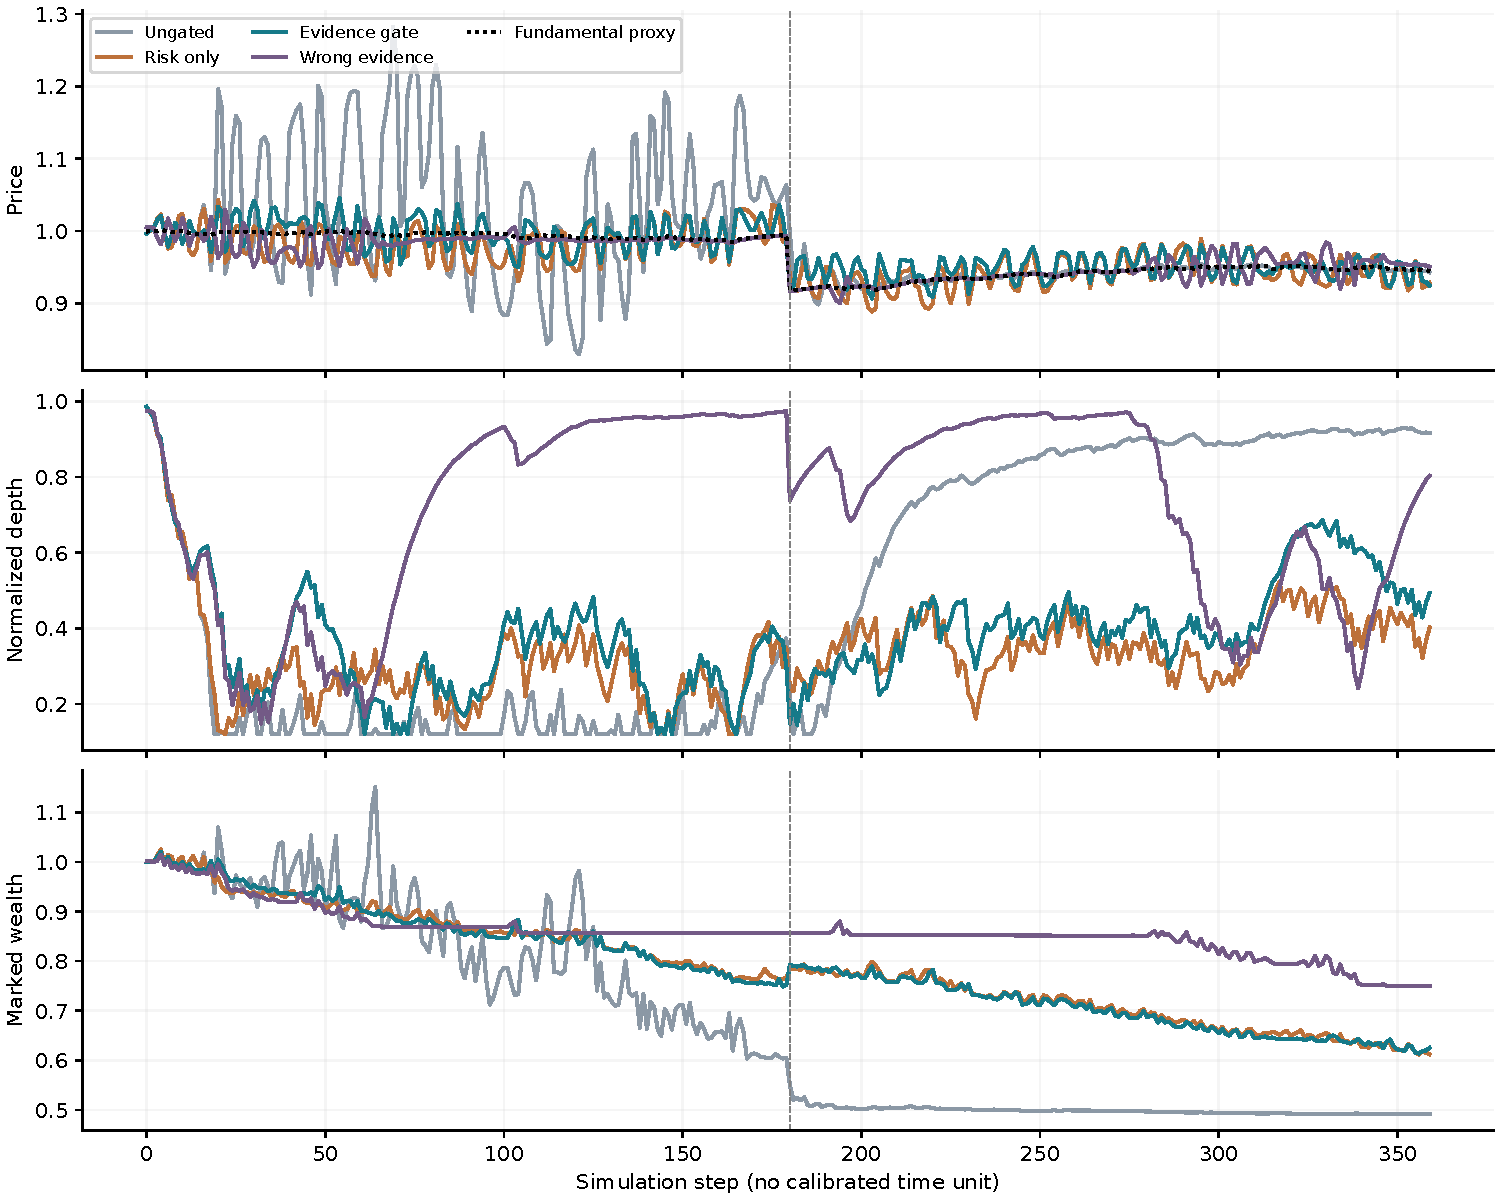
\includegraphics[width=\linewidth]{manuscript/figures/market_paths.pdf}
\caption{Prespecified replication index zero in the high-coupling shock scenario. Paths illustrate mechanisms, not an average or a selected best case. The vertical marker denotes the shock.}
\end{figure}

\subsection{Numerical sensitivity and uncertainty}
The return cap can change extreme paths. We rerun the high-coupling, correlated, fast, leveraged scenario at caps 0.125, 0.25, and 0.5 with and without shock. This post-audit diagnostic is separate from the primary grid. It tests a numerical boundary rather than calibrating a crisis model.
\begin{table}[htbp]\centering\small
\begin{tabular}{rlrrr}\toprule
Return cap & Policy & Net return (\%) & Dislocation (\%) & Clipped steps\\\midrule
0.125 & Evidence gate & -34.48 & 0.00 & 0.000\\
0.125 & Risk only & -34.92 & 0.00 & 0.000\\
0.125 & Ungated & 936957.46 & 70.31 & 63.312\\
0.125 & Wrong evidence & -11.64 & 0.00 & 0.000\\
0.250 & Evidence gate & -34.48 & 0.00 & 0.000\\
0.250 & Risk only & -34.92 & 0.00 & 0.000\\
0.250 & Ungated & -37.13 & 32.81 & 0.688\\
0.250 & Wrong evidence & -11.64 & 0.00 & 0.000\\
0.500 & Evidence gate & -34.48 & 0.00 & 0.000\\
0.500 & Risk only & -34.92 & 0.00 & 0.000\\
0.500 & Ungated & -36.02 & 29.69 & 0.000\\
0.500 & Wrong evidence & -11.64 & 0.00 & 0.000\\
\bottomrule\end{tabular}
\caption{Post-audit cap sensitivity in the high-coupling shock case. Clipped steps count the entire trajectory, including initialization.}
\end{table}

Monte Carlo errors use independent replication indices, not time steps. Paired differences use matched scenarios and seeds. Grid averages are descriptive under uniform weighting of the chosen settings, not expected returns under an estimated market distribution.

The networks are trained once. Simulation errors are conditional on those weights, parameters, and equations. Training-seed variation, model selection, environment misspecification, and uncertainty about real participant behavior are not included.

\section{What the experiments establish about market transitions}
The completed evidence supports a conditional mechanism story. Correlated orders can interact with leverage and thin liquidity; a model can protect capital by trading less; and that protection can coexist with delayed liquidity recovery. It does not prove that AI financial models will cause a real crash.

Interpretability must be tested behaviorally. A policy with incorrect assumptions can trade less and lose less. Ranking architectures by return alone could reward withdrawal while concealing inferior inference. Forecast loss, exposure, turnover, cost, and market externalities belong in the same evaluation.

There is no universal operating speed. In a richer environment it depends on information half-life, depth, queue position, inference latency, capital, and others' responses. Faster action can capture a fleeting signal or cause repeated costly reversals. Here $\eta$ is a fraction per abstract step; translating it into milliseconds is unsupported.

The grid also does not locate a real-world saturation point. A transition surface requires finer interventions, uncertainty bounds, and held-out environments. Thresholds can disappear when the participant mix, background response, or impact law changes.

\section{Validation program for alpha preservation and systemic effects}
\subsection{A population that tests the intended claim}
A next experiment should place CMTF alongside factor models, regularized predictors, recurrent or attention-based time-series models, reinforcement-learning policies, and constrained market makers. Composition must vary rather than replacing every participant with the same architecture. Capital concentration should vary at fixed total capital, separately from model count.

Baselines need the same inputs and risk controls. Remove regime conditioning, evidence gating, causal feature interfaces, abstention, and outcome learning separately. Randomized abstention matched for exposure and turnover tests whether a gain comes from information selection or lower activity.

\subsection{Identification inside and outside a simulator}
Within a simulator, fixed shock paths support interventions on populations. At shock level $s$, the effect on outcome $Y$ is
\[
\Delta_Y(s)=\E[Y\mid do(\Pi=\Pi_1),s]-\E[Y\mid do(\Pi=\Pi_0),s].
\]
Population $\Pi$ (capital pi) specifies composition, allocation, and shared constraints. The interaction with shock is $\Delta_Y(s_1)-\Delta_Y(s_0)$. The intervention must specify what changes and what remains fixed.

Historical attribution needs more than a correlation between estimated AI activity and volatility. Adoption can respond to the same conditions that move volatility. A credible design would require exogenous variation, measurement-error treatment, and assumptions about spillovers. This manuscript does not claim such identification.

\subsection{Proposed endpoints}
For alpha preservation, prespecify factors, financing, turnover, impact, and inference cost. Estimate out-of-sample net alpha in sequential windows, retaining negative windows. For a decay rate, fit a declared model to the same signal across controlled competing-capital interventions, with uncertainty clustered by seed and episode.

For adaptation, measure detection delay, false alarms, and regime-probability calibration. For stability, distinguish drawdowns from fundamental dislocations, measure spread and depth, inspect forced liquidation, and retain censored recovery paths. For interpretability, test decision reconstruction and interventions on recorded assumptions.

These endpoints are a protocol, not completed results. That distinction makes the manuscript reviewable without converting future experiments into past-tense evidence.

\section{Engineering implications and FPGA-oriented partition}
A field-programmable gate array (FPGA) is reconfigurable hardware for bounded arithmetic and control logic. The proposed partition keeps neural inference, graph authoring, estimation, and training on general-purpose or accelerator hardware. Timestamp comparisons, numeric checks, masks, bounded normalization, and order limits could use an FPGA interface.

The potential benefit is predictable execution of a small verified contract. This does not move open-ended causal reasoning into logic gates or eliminate ingestion delay. Fixed-point precision, overflow, synchronization, atomic updates, and software fallback need validation.

A hardware claim should report device, clock, precision, synthesis tools, resources, power, end-to-end latency, and software-equivalence tests. None is measured here. The contribution is an interface specification and validation plan.

\section{Limitations and reproducibility}
All public numerical results use generated data. Experiment I supplies oracle regimes and filter parameters. Experiment II has homogeneous capital, small fixed experts, simplified impact and liquidity, and no order book. Its gate checks predictive proxies rather than formally identifying macroeconomic effects.

The design is exploratory, without a prospective benchmark, rare-crisis power analysis, or comprehensive hyperparameter search. Exposure-matched abstention and diverse learned populations remain untested. Results motivate further experiments; they do not establish superiority to contemporary financial models.

Private operational records inform a confidential validation edition. They are excluded from public numerical claims because the public package cannot reproduce the deployment or verify complete marked-to-market equity. The source package: \begin{quote}
\small\raggedright
\def\UrlBreaks{\do\/\do-}
\url{https://github.com/timi-le/Market-Transitions-under-AI-Financial-Models}\end{quote} contains configurations, replication-level results, figures, tests, and build commands. No broker connection, credential, or private repository is required for public reproduction. Small floating-point differences can occur across numerical-library versions.

\subsection{Authorship}
The author develops ATRX Intelligence and CMTF.

\section{Conclusion}
The central transition is from evaluating one model against a fixed market to evaluating a population that changes the market. CMTF expresses and exposes assumptions connecting neural proposals to mechanisms and decisions. Its usefulness must be tested by separating information quality, risk reduction, and collective feedback.

The completed diagnostics show conditional benefits of regime averaging and failure under misspecification. Fewer dislocations and smaller losses can arise without better forecasts; individual protection can coexist with poor liquidity recovery. Positive alpha, real-market thresholds, and calibrated crash forecasts remain unestablished. A credible account of continuous adaptability must include these failure cases alongside its intended benefits.

\begin{thebibliography}{9}
\bibitem{perdomo} J. Perdomo, T. Zrnic, C. Mendler-D\"unner, and M. Hardt. Performative Prediction. \emph{ICML}, PMLR 119, pp. 7599--7609, 2020. \url{https://proceedings.mlr.press/v119/perdomo20a.html}.
\bibitem{shazeer} N. Shazeer, A. Mirhoseini, K. Maziarz, A. Davis, Q. Le, G. Hinton, and J. Dean. Outrageously Large Neural Networks: The Sparsely-Gated Mixture-of-Experts Layer. 2017. \url{https://arxiv.org/abs/1701.06538}.
\bibitem{dowhy} A. Sharma and E. Kiciman. DoWhy: An End-to-End Library for Causal Inference. 2020. \url{https://arxiv.org/abs/2011.04216}.
\bibitem{abides} D. Byrd, M. Hybinette, and T. H. Balch. ABIDES: Towards High-Fidelity Market Simulation for AI Research. 2019. \url{https://arxiv.org/abs/1904.12066}.
\bibitem{narang} A. Narang, E. Faulkner, D. Drusvyatskiy, M. Fazel, and L. J. Ratliff. Multiplayer Performative Prediction: Learning in Decision-Dependent Games. arXiv preprint, 2022. \url{https://arxiv.org/abs/2201.03398}.
\bibitem{thurner} S. Thurner, J. D. Farmer, and J. Geanakoplos. Leverage Causes Fat Tails and Clustered Volatility. arXiv preprint, 2009, revised 2010. \url{https://arxiv.org/abs/0908.1555}.
\bibitem{kirilenko} A. Kirilenko, A. S. Kyle, M. Samadi, and T. Tuzun. The Flash Crash: The Impact of High Frequency Trading on an Electronic Market. Working paper, version of 5 May 2014. \url{https://www.cftc.gov/sites/default/files/idc/groups/public/@economicanalysis/documents/file/oce_flashcrash0314.pdf}.


\end{thebibliography}

